% Public source snapshot: a third-party textbook reference has been omitted.
% See sources/README.md for the project's stricter independent-provenance and
% licensing boundary.
\documentclass{article}
\usepackage{graphicx}
\usepackage{amsmath}
\usepackage{amssymb}
\usepackage{listings}
\usepackage[margin=1in]{geometry}
\usepackage{xcolor}
\usepackage{tikz}
\usetikzlibrary{shapes, arrows, positioning, calc, decorations.pathreplacing}
\usepackage{tcolorbox}
\usepackage{booktabs}

% Define colors for syntax highlighting
\definecolor{codegreen}{rgb}{0,0.6,0}
\definecolor{codegray}{rgb}{0.5,0.5,0.5}
\definecolor{codepurple}{rgb}{0.58,0,0.82}
\definecolor{backcolour}{rgb}{0.95,0.95,0.92}

% Python style for highlighting
\lstdefinestyle{pythonstyle}{
    backgroundcolor=\color{backcolour},
    commentstyle=\color{codegreen},
    keywordstyle=\color{magenta},
    numberstyle=\tiny\color{codegray},
    stringstyle=\color{codepurple},
    basicstyle=\ttfamily\footnotesize,
    breakatwhitespace=false,
    breaklines=true,
    captionpos=b,
    keepspaces=true,
    numbers=left,
    numbersep=5pt,
    showspaces=false,
    showstringspaces=false,
    showtabs=false,
    tabsize=2
}
\lstset{style=pythonstyle}

\title{Lecture 11: Pre-trained Language Models and Self-Supervised Learning}
\author{Deep Learning Class}
\date{\today}

\begin{document}
\maketitle

In the last lecture, you saw Vision Transformers. But here's the secret: ViT only exists because of what we're about to learn today. BERT (2018) proved that Transformers + pre-training = breakthrough. ViT (2020) took that proven recipe and asked: ``Can we do this for images too?'' Today, we'll learn about the NLP revolution that made ViT possible.

\begin{tcolorbox}[colback=blue!5!white, colframe=blue!75!black, title=Lecture Arc]
Today's journey from specialized Transformers to foundation models:

\begin{enumerate}
\item Motivation: The transfer learning revolution in computer vision
\item Can we do the same for text? The pre-training paradigm
\item Three architectural families: BERT (encoder), GPT (decoder), T5 (encoder-decoder)
\item Pre-training objectives: MLM, CLM, and span corruption
\item The fine-tuning paradigm: Adapt pre-trained models to specific tasks
\item In-context learning: The emergence of zero-parameter adaptation
\item Why self-supervision works differently for vision vs. language
\item The evolution of transfer learning: From ImageNet to foundation models
\end{enumerate}
\end{tcolorbox}

\section{Motivation: The Transfer Learning Revolution}

\subsection{The Computer Vision Story}

Let us start with a story from computer vision that transformed the field.

\textbf{The year is 2012}. You want to build a classifier to recognize different types of flowers. You have:
\begin{itemize}
\item A dataset of 5,000 flower images (carefully labeled by hand)
\item A deep neural network architecture (let's say, a CNN with 50 million parameters)
\item A GPU and a few days of compute
\end{itemize}

\textbf{Question}: Should you train your network from scratch on these 5,000 images?

\textbf{Answer in 2012}: Probably not. Your model will overfit badly. You need hundreds of thousands of images to train a deep network from scratch.

But wait---someone else has already trained a deep CNN on ImageNet!

\begin{center}
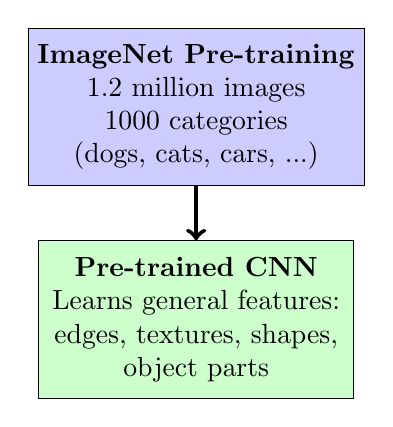
\begin{tikzpicture}[scale=0.9]
% ImageNet pre-training
\node[draw, rectangle, minimum width=4cm, minimum height=2cm, fill=blue!20, align=center] (imagenet) at (0,3)
   {\textbf{ImageNet Pre-training}\\1.2 million images\\1000 categories\\(dogs, cats, cars, ...)};

\node[draw, rectangle, minimum width=4cm, minimum height=2cm, fill=green!20, align=center] (pretrained) at (0,0)
   {\textbf{Pre-trained CNN}\\Learns general features:\\edges, textures, shapes,\\object parts};

\draw[->, ultra thick] (imagenet) -- (pretrained);
\end{tikzpicture}
\end{center}

\textbf{The key insight}: The features learned on ImageNet (edge detectors in early layers, texture recognizers in middle layers, part detectors in late layers) are \textit{general}. They transfer to new tasks!

\subsection{Transfer Learning in Action}

Here's what you do:

\begin{center}
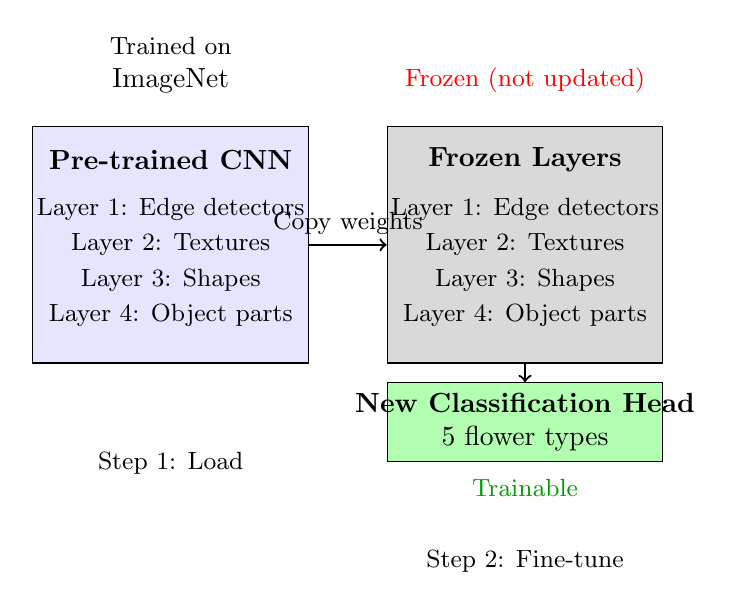
\begin{tikzpicture}[scale=0.9, node distance=1.5cm]
% Step 1: Take pre-trained model
\node[draw, rectangle, minimum width=3.5cm, minimum height=3cm, fill=blue!10] (pretrained) at (0,0) {};
\node[align=center] at (0, 1.2) {\textbf{Pre-trained CNN}};
\node[align=center, font=\small] at (0, 0.5) {Layer 1: Edge detectors};
\node[align=center, font=\small] at (0, 0) {Layer 2: Textures};
\node[align=center, font=\small] at (0, -0.5) {Layer 3: Shapes};
\node[align=center, font=\small] at (0, -1) {Layer 4: Object parts};

\node[above=0.3cm of pretrained, align=center] {\small Trained on\\ImageNet};

% Step 2: Freeze early layers
\node[draw, rectangle, minimum width=3.5cm, minimum height=3cm, fill=gray!30] (frozen) at (5,0) {};
\node[align=center] at (5, 1.2) {\textbf{Frozen Layers}};
\node[align=center, font=\small] at (5, 0.5) {Layer 1: Edge detectors};
\node[align=center, font=\small] at (5, 0) {Layer 2: Textures};
\node[align=center, font=\small] at (5, -0.5) {Layer 3: Shapes};
\node[align=center, font=\small] at (5, -1) {Layer 4: Object parts};

\node[above=0.3cm of frozen, red, font=\small] {Frozen (not updated)};

% Step 3: Add new head
\node[draw, rectangle, minimum width=3.5cm, minimum height=1cm, fill=green!30] (head) at (5, -2.5) {};
\node[align=center] at (5, -2.5) {\textbf{New Classification Head}\\5 flower types};
\node[below=0.1cm of head, green!60!black, font=\small] {Trainable};

% Arrows
\draw[->, thick] (pretrained) -- (frozen) node[midway, above] {\small Copy weights};
\draw[->, thick] (frozen) -- (head);

% Labels
\node[below=1cm of pretrained] {\small Step 1: Load};
\node[below=1cm of head] {\small Step 2: Fine-tune};
\end{tikzpicture}
\end{center}

\textbf{What happens during fine-tuning}:
\begin{enumerate}
\item Take the pre-trained CNN
\item \textit{Freeze} the early layers (edge/texture detectors are universal!)
\item Replace the final classification layer (1000 ImageNet classes $\rightarrow$ 5 flower types)
\item Train on your 5,000 flower images
\begin{itemize}
\item Only the final layer gets updated
\item Or: fine-tune the entire network with a very small learning rate
\end{itemize}
\end{enumerate}

\textbf{The result}: With just 5,000 images, you achieve excellent performance! The pre-trained features do most of the work.

\subsection{Why Does This Work?}

\begin{tcolorbox}[colback=green!5!white, colframe=green!50!black, title=The Hierarchy of Visual Features]
Deep networks learn a \textbf{hierarchy of features}:

\begin{itemize}
\item \textbf{Layer 1}: Edge detectors (horizontal, vertical, diagonal)
\begin{itemize}
\item These are useful for \textit{any} image task!
\item Whether you're recognizing flowers, cars, or medical scans, you need edge detection
\end{itemize}

\item \textbf{Layer 2}: Texture recognizers (stripes, dots, gradients)
\begin{itemize}
\item Still very general---most objects have textures
\end{itemize}

\item \textbf{Layer 3}: Shape and pattern detectors (circles, squares, complex curves)
\begin{itemize}
\item Getting more specific, but still broadly useful
\end{itemize}

\item \textbf{Layer 4}: Object part detectors (wheels, faces, petals)
\begin{itemize}
\item Task-specific features start appearing here
\end{itemize}

\item \textbf{Final layer}: Class predictions (dog breeds, car models, flower types)
\begin{itemize}
\item Completely task-specific---this is what we replace
\end{itemize}
\end{itemize}

\textbf{Transfer learning works because the early layers learn general features that are useful across many tasks.}
\end{tcolorbox}

\subsection{The Impact on Computer Vision}

This discovery transformed computer vision:

\begin{itemize}
\item \textbf{Before}: Every new task required training from scratch on massive datasets
\item \textbf{After}: Pre-train once on ImageNet, then fine-tune on small task-specific datasets
\end{itemize}

\textbf{Practical benefits}:
\begin{itemize}
\item Medical imaging: Fine-tune on 1,000 X-rays instead of needing 100,000
\item Satellite imagery: Fine-tune on a few thousand images
\item Industrial inspection: Fine-tune on small defect datasets
\item Any specialized domain: Can now use deep learning with limited data!
\end{itemize}

By 2015, transfer learning was standard practice in computer vision. Every vision researcher used pre-trained ImageNet models.

\subsection{The Natural Question for NLP}

\begin{center}
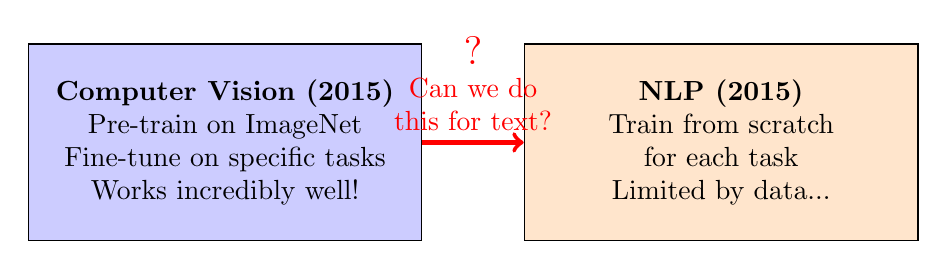
\begin{tikzpicture}[scale=0.9]
\node[draw, rectangle, minimum width=5cm, minimum height=2.5cm, fill=blue!20, align=center] (vision) at (0,0)
   {\textbf{Computer Vision (2015)}\\Pre-train on ImageNet\\Fine-tune on specific tasks\\Works incredibly well!};

\node[draw, rectangle, minimum width=5cm, minimum height=2.5cm, fill=orange!20, align=center] (nlp) at (7,0)
   {\textbf{NLP (2015)}\\Train from scratch\\for each task\\Limited by data...};

\draw[->, ultra thick, red] (vision) -- (nlp) node[midway, above, align=center] {\Large ?\\Can we do\\this for text?};
\end{tikzpicture}
\end{center}

\textbf{The analogy seems compelling}:
\begin{itemize}
\item Images have edges, textures, shapes (general features)
\item Text has grammar, syntax, semantics (general linguistic features)
\item If we can pre-train on general image data, why not pre-train on general text data?
\end{itemize}

\textbf{But there's a critical difference}: What is the equivalent of ImageNet for text? And more fundamentally, what task should we use for pre-training?

\section{The Pre-Training Revolution: Transfer Learning for Text}

\subsection{The Challenge: What Should We Pre-train On?}

In computer vision, ImageNet provided:
\begin{itemize}
\item 1.2 million labeled images
\item 1000 object categories
\item A clear task: classify images
\end{itemize}

\textbf{For text, we don't have a comparable labeled dataset}. Creating one would require:
\begin{itemize}
\item Millions of labeled text examples
\item Diverse tasks (sentiment, QA, classification, etc.)
\item Enormous human annotation effort (years of work, millions of dollars)
\end{itemize}

\textbf{But wait}---do we even \textit{need} labels?

\subsection{The Key Insight: Self-Supervised Learning}

Here's the brilliant realization:

\begin{tcolorbox}[colback=yellow!5!white, colframe=orange!50!black, title=Text Contains Its Own Supervision Signal]
We have access to \textbf{unlimited unlabeled text}:
\begin{itemize}
\item Wikipedia: billions of tokens
\item Books: billions of tokens
\item Web pages: trillions of tokens
\item News, forums, code: trillions more
\end{itemize}

And text has \textbf{inherent structure}:
\begin{itemize}
\item If we hide a word, can the model predict it from context?
\item If we give the first half of a sentence, can the model generate the second half?
\item These tasks don't need human labels---the text itself provides the ``labels''!
\end{itemize}

This is called \textbf{self-supervised learning}: creating supervised tasks from unlabeled data.
\end{tcolorbox}

\subsubsection{Why Self-Supervised Learning Works Better for Text Than Images (Initially)}

This is a crucial insight that explains why the NLP breakthrough came before similar breakthroughs in computer vision.

\textbf{The fundamental difference: Discrete vs. Continuous}

\begin{center}
\begin{tabular}{p{5cm}p{5cm}}
\toprule
\textbf{Text (Discrete)} & \textbf{Images (Continuous)} \\
\midrule
Finite vocabulary ($\sim$30K--50K tokens) & ``Infinite vocabulary'' (pixel values: $256^3$ colors) \\
\midrule
Natural prediction task: ``What word comes next?'' & Unnatural prediction: ``What are the exact pixel values?'' \\
\midrule
Cross-entropy loss works perfectly & Regression loss is noisy, pixels have weak individual meaning \\
\midrule
Predicting one token provides strong signal & Predicting exact pixels provides weak signal \\
\midrule
Tokens are semantically meaningful units & Individual pixels are not semantically meaningful \\
\bottomrule
\end{tabular}
\end{center}

\textbf{Why this matters}:

\begin{itemize}
\item \textbf{For text}: If you hide the word ``cat'' and the model predicts ``dog'', that's semantically similar---the model learned something useful even when wrong!

\item \textbf{For images}: If you hide a pixel with value RGB(127, 45, 200) and the model predicts RGB(125, 47, 198), did it learn anything useful? The relationship between pixel values and semantics is indirect.

\item \textbf{Prediction as a task}:
\begin{itemize}
\item Text: ``The cat sat on the \_\_\_'' $\rightarrow$ ``mat'' (clear, natural task)
\item Images: ``Predict pixel (100, 200) given all other pixels'' (unnatural, weak supervision)
\end{itemize}
\end{itemize}

\begin{tcolorbox}[colback=blue!5!white, colframe=blue!75!black, title=The Historical Development]
\textbf{Timeline of self-supervised learning}:

\begin{enumerate}
\item \textbf{2013--2017}: Word2Vec, GloVe use word co-occurrence (limited SSL for text)

\item \textbf{2018}: BERT breakthrough---full self-supervised pre-training for text works spectacularly

\item \textbf{2018--2020}: Computer vision researchers ask: ``Can we do this for images?''

\item \textbf{2020+}: Vision SSL breakthroughs, but using \textit{different} techniques:
\begin{itemize}
\item \textbf{Contrastive learning} (SimCLR, MoCo): Don't predict pixels; instead learn that augmented views of same image are similar
\item \textbf{Masked autoencoding} (MAE): Like BERT for images, but with large patches (not pixels)
\item \textbf{CLIP}: Use text as supervision for images (multimodal)
\end{itemize}
\end{enumerate}

\textbf{Key insight}: Vision SSL had to work around the ``infinite vocabulary'' problem. Text SSL could use the natural discrete structure directly.
\end{tcolorbox}

\textbf{Modern perspective}: We \textit{can} do SSL for both modalities now, but text's discrete nature made the path more straightforward. Vision SSL required creative solutions:

\begin{itemize}
\item \textbf{Contrastive learning}: Instead of predicting pixels, learn invariances (``these two augmented views are the same image'')
\item \textbf{Tokenization}: Break images into discrete ``tokens'' (like ViT does), then treat more like text
\item \textbf{Large patches}: MAE masks 16x16 patches, not individual pixels
\item \textbf{Vector quantization}: VQ-VAE creates discrete ``codebook'' of visual patterns
\end{itemize}

The key lesson: \textbf{Self-supervised learning needs the right inductive bias for each modality}. Text's discrete tokens were a gift; vision required more engineering.

\textbf{Examples of self-supervision in text}:

\begin{enumerate}
\item \textbf{Masked Language Modeling}:
\begin{itemize}
\item Original: ``I love this red car''
\item Hide a word: ``I love this [MASK] car''
\item Task: Predict ``red''
\item \textit{No human labels needed---the original text is the label!}
\end{itemize}

\item \textbf{Next Token Prediction}:
\begin{itemize}
\item Given: ``The cat sat on the''
\item Task: Predict ``mat''
\item \textit{Again, the text itself provides the answer!}
\end{itemize}

\item \textbf{Sentence Ordering}:
\begin{itemize}
\item Shuffle sentences: ``[3] He went home. [1] John woke up. [2] He had breakfast.''
\item Task: Restore the correct order
\item \textit{The original document tells us the right order!}
\end{itemize}
\end{enumerate}

\subsection{The Two-Stage Paradigm}

Just like in computer vision, we now have a two-stage approach:

\begin{center}
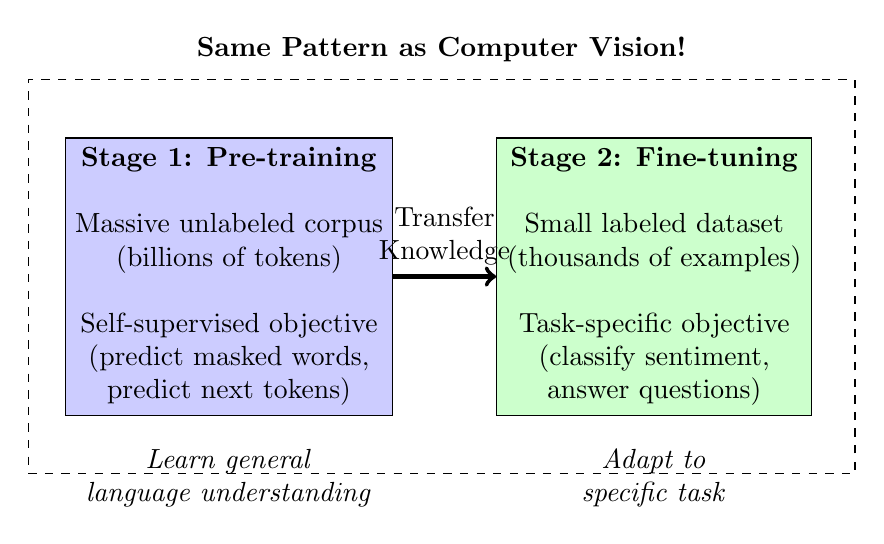
\begin{tikzpicture}[scale=0.9, node distance=2.5cm]
% Stage 1: Pre-training
\node[draw, rectangle, minimum width=4cm, minimum height=3cm, fill=blue!20, align=center] (pretrain) at (0,0)
   {\textbf{Stage 1: Pre-training}\\\\Massive unlabeled corpus\\(billions of tokens)\\\\Self-supervised objective\\(predict masked words,\\predict next tokens)};

% Stage 2: Fine-tuning
\node[draw, rectangle, minimum width=4cm, minimum height=3cm, fill=green!20, align=center] (finetune) at (6,0)
   {\textbf{Stage 2: Fine-tuning}\\\\Small labeled dataset\\(thousands of examples)\\\\Task-specific objective\\(classify sentiment,\\answer questions)};

\draw[->, ultra thick] (pretrain) -- (finetune) node[midway, above, align=center] {Transfer\\Knowledge};

\node[align=center, below=0.3cm of pretrain] {\textit{Learn general}\\\textit{language understanding}};
\node[align=center, below=0.3cm of finetune] {\textit{Adapt to}\\\textit{specific task}};

% Analogy box
\node[draw, rectangle, dashed, minimum width=10.5cm, minimum height=5cm] (box) at (3, 0) {};
\node[above=0.1cm of box, fill=white] {\textbf{Same Pattern as Computer Vision!}};
\end{tikzpicture}
\end{center}

\textbf{Pre-training} (analogous to ImageNet training):
\begin{itemize}
\item Train on massive unlabeled text
\item Self-supervised objective (e.g., predict masked words)
\item Model learns general linguistic knowledge:
\begin{itemize}
\item Syntax and grammar
\item Word meanings and relationships
\item World knowledge and facts
\item Discourse structure
\end{itemize}
\end{itemize}

\textbf{Fine-tuning} (analogous to adapting to flower classification):
\begin{itemize}
\item Take the pre-trained model
\item Add a task-specific head
\item Train on small labeled dataset for your specific task
\item The linguistic knowledge transfers!
\end{itemize}

\subsection{The Breakthrough Moment}

\textbf{2018}: Three papers demonstrated this paradigm works spectacularly well for text:

\begin{enumerate}
\item \textbf{ELMo} (Peters et al.): Pre-trained contextualized word embeddings

\item \textbf{ULMFiT} (Howard \& Ruder): Showed how to fine-tune language models effectively

\item \textbf{BERT} (Devlin et al.): The breakthrough that changed everything
\begin{itemize}
\item Pre-trained a Transformer encoder on masked language modeling
\item Fine-tuned on 11 different NLP tasks
\item Achieved state-of-the-art on \textit{all of them}
\item Often with just a few thousand labeled examples!
\end{itemize}
\end{enumerate}

\begin{tcolorbox}[colback=red!5!white, colframe=red!75!black, title=The Impact]
Just like ImageNet pre-training transformed computer vision in 2012, pre-trained Transformers transformed NLP in 2018.

\textbf{Before 2018}:
\begin{itemize}
\item Each task required its own architecture
\item Needed large labeled datasets (often unavailable)
\item Performance limited by task-specific data
\end{itemize}

\textbf{After 2018}:
\begin{itemize}
\item One pre-trained model works for many tasks
\item Can achieve strong performance with small labeled datasets
\item Transfer learning is the default approach
\end{itemize}

By 2019, \textit{no one} was training NLP models from scratch anymore (unless they had a very good reason).
\end{tcolorbox}

\subsection{Why This Wasn't Obvious}

You might wonder: ``Why did it take so long? The idea seems obvious in hindsight!''

Several factors delayed the breakthrough:

\begin{enumerate}
\item \textbf{Computational barriers}: Pre-training large models on billions of tokens requires substantial compute (GPUs/TPUs) that only became accessible around 2017--2018

\item \textbf{Architecture}: RNNs (dominant pre-2017) are hard to parallelize and don't scale well. Transformers (2017) made large-scale pre-training practical

\item \textbf{Belief in supervised learning}: The field was focused on getting more labeled data, not leveraging unlabeled data

\item \textbf{Task-specific mindset}: Researchers built specialized architectures for each task, rather than seeking general-purpose models

\item \textbf{Discrete vs. continuous}: Text's discrete nature made SSL more natural, but this wasn't fully appreciated until the breakthrough
\end{enumerate}

The convergence of (1) scalable architectures (Transformers), (2) available compute, (3) self-supervised objectives, and (4) understanding of text's discrete advantage created the breakthrough.

\subsection{The Road Ahead for This Lecture}

Now that we understand \textit{why} pre-training matters (transfer learning from unlabeled data using self-supervision), we can address:

\begin{enumerate}
\item \textbf{How} to pre-train: What objectives work? What architectures?
\item \textbf{Specialization}: BERT vs. GPT vs. T5---why three families?
\item \textbf{Scaling}: How big should models be? How much data?
\item \textbf{Efficient adaptation}: Can we avoid fine-tuning all parameters?
\end{enumerate}

But first, let us make the analogy between computer vision and NLP transfer learning completely explicit.

\subsection{The Complete Analogy: CV Transfer Learning $\leftrightarrow$ NLP Pre-training}

Understanding this parallel is crucial for grasping why pre-trained language models work.

\begin{center}
\begin{tabular}{p{5.5cm}p{5.5cm}}
\toprule
\textbf{Computer Vision (ImageNet)} & \textbf{NLP (Pre-trained LMs)} \\
\midrule
\multicolumn{2}{c}{\textit{Stage 1: Pre-training on General Data}} \\
\midrule
Train CNN on ImageNet (1.2M images, 1000 classes) & Train Transformer on web text (billions of tokens) \\
\midrule
Supervised: predict image labels & Self-supervised: predict masked/next tokens \\
\midrule
Learns general visual features: edges $\rightarrow$ textures $\rightarrow$ shapes $\rightarrow$ object parts & Learns general linguistic features: syntax $\rightarrow$ semantics $\rightarrow$ world knowledge \\
\midrule
Takes days/weeks on GPUs & Takes weeks/months on many GPUs \\
\midrule
Done once, then reused & Done once, then reused \\
\midrule
\multicolumn{2}{c}{\textit{Stage 2: Adaptation to Specific Tasks}} \\
\midrule
Replace final layer (1000 classes $\rightarrow$ 5 flower types) & Add task-specific head or use prompting \\
\midrule
Fine-tune on small dataset (5,000 flower images) & Fine-tune on small dataset (5,000 sentiment examples) or few-shot prompt \\
\midrule
Freeze early layers or fine-tune all with small LR & Fine-tune all layers with small LR, or no updates (in-context) \\
\midrule
Takes hours & Takes hours (fine-tuning) or seconds (prompting) \\
\midrule
\multicolumn{2}{c}{\textit{What Gets Transferred}} \\
\midrule
Edge detectors, texture recognizers, shape detectors & Grammar rules, semantic relationships, world knowledge \\
\midrule
Visual ``understanding'' & Language ``understanding'' \\
\midrule
Low/mid-level features are universal & Linguistic features are universal \\
\midrule
\multicolumn{2}{c}{\textit{The Key Benefit}} \\
\midrule
Strong performance with 5,000 images instead of 500,000 & Strong performance with 5,000 examples instead of 500,000 \\
\midrule
General features do most of the work & General linguistic knowledge does most of the work \\
\midrule
\multicolumn{2}{c}{\textit{The Key Difference}} \\
\midrule
Pre-training requires supervised labels (ImageNet annotations) & Pre-training uses self-supervision (text provides its own labels) \\
\midrule
Finite, curated dataset (ImageNet) & Unlimited data (entire internet) \\
\bottomrule
\end{tabular}
\end{center}

\begin{tcolorbox}[colback=blue!5!white, colframe=blue!75!black, title=The Crucial Advantage of NLP]
\textbf{Why NLP pre-training is even more powerful}:

\begin{enumerate}
\item \textbf{Unlimited data}: ImageNet has 1.2M images (expensive to label). Text? We can use trillions of tokens from the web, books, code---all unlabeled!

\item \textbf{Self-supervision}: ImageNet required years of human labeling. Text creates its own labels (predict masked/next token).

\item \textbf{Scaling}: Because data is unlimited and free, we can scale to massive sizes (GPT-3: 175B parameters trained on 300B+ tokens).

\item \textbf{Generalization}: At sufficient scale, models can perform new tasks zero-shot (in-context learning)---going beyond traditional transfer learning!
\end{enumerate}
\end{tcolorbox}

\textbf{The Evolution of Adaptation Strategies}

\begin{center}
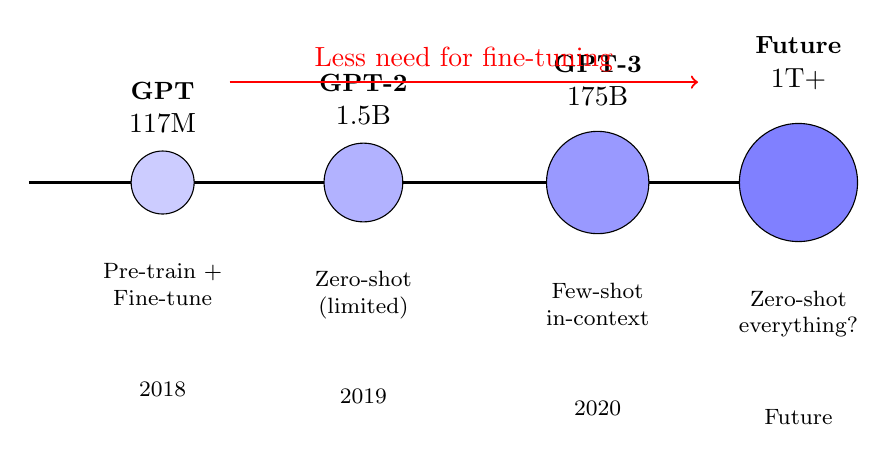
\begin{tikzpicture}[scale=0.85]
% Timeline
\draw[->, thick] (0,0) -- (12,0);

% GPT (2018)
\node[draw, circle, fill=blue!20, minimum size=0.8cm] (gpt) at (2,0) {};
\node[above=0.1cm of gpt, align=center] {\small \textbf{GPT}\\117M};
\node[below=0.5cm of gpt, align=center, font=\footnotesize] {Pre-train +\\Fine-tune};

% GPT-2 (2019)
\node[draw, circle, fill=blue!30, minimum size=1cm] (gpt2) at (5,0) {};
\node[above=0.1cm of gpt2, align=center] {\small \textbf{GPT-2}\\1.5B};
\node[below=0.5cm of gpt2, align=center, font=\footnotesize] {Zero-shot\\(limited)};

% GPT-3 (2020)
\node[draw, circle, fill=blue!40, minimum size=1.3cm] (gpt3) at (8.5,0) {};
\node[above=0.2cm of gpt3, align=center] {\small \textbf{GPT-3}\\175B};
\node[below=0.5cm of gpt3, align=center, font=\footnotesize] {Few-shot\\in-context};

% Future
\node[draw, circle, fill=blue!50, minimum size=1.5cm] (future) at (11.5,0) {};
\node[above=0.3cm of future, align=center] {\small \textbf{Future}\\1T+};
\node[below=0.5cm of future, align=center, font=\footnotesize] {Zero-shot\\everything?};

% Labels
\node[below=2cm of gpt, font=\footnotesize] {2018};
\node[below=2cm of gpt2, font=\footnotesize] {2019};
\node[below=2cm of gpt3, font=\footnotesize] {2020};
\node[below=2cm of future, font=\footnotesize] {Future};

% Arrow annotation
\draw[->, thick, red] (3, 1.5) -- (10, 1.5) node[midway, above, align=center] {Less need for fine-tuning};
\end{tikzpicture}
\end{center}

The trend: As models scale, they need less task-specific adaptation. The ultimate transfer learning is no adaptation at all---just prompting!

Let us start with the architectural choices and self-supervised objectives.

\section{Deep Dive: Architectures and Self-Supervised Learning Objectives}

\subsection{Introduction: The Landscape of Self-Supervision}

We've seen that pre-training on massive unlabeled data is the foundation of modern NLP. But \textit{how} exactly do we create a learning signal from raw text, and how does the model architecture influence this process?

\textbf{The core challenge}: Text has no inherent labels. We need to design \textbf{pretext tasks}---artificial objectives that force the model to learn useful representations.

\begin{tcolorbox}[colback=blue!5!white, colframe=blue!75!black, title=What Makes a Good SSL Objective?]
A good self-supervised objective should:

\begin{enumerate}
\item \textbf{Require understanding}: Force the model to learn linguistic patterns, not memorize
\item \textbf{Be efficient}: Use compute and data effectively
\item \textbf{Align with downstream tasks}: The pretext task should teach skills needed for real tasks
\item \textbf{Scale well}: Work with billions of parameters and trillions of tokens
\end{enumerate}
\end{tcolorbox}

The choice of objective is deeply intertwined with the model's architecture. The Transformer architecture is modular, and by utilizing the encoder, the decoder, or both, we arrive at three distinct families, each optimized for different objectives and tasks.

\subsubsection{The Three Architectural Families}

The key distinction lies in the attention patterns they employ:

\begin{itemize}
\item \textbf{Bidirectional attention} (Encoder): Every token can attend to every other token (including future tokens). Ideal for understanding tasks.
\item \textbf{Causal attention} (Decoder): Each token can only attend to past tokens (masked self-attention). Essential for autoregressive generation.
\end{itemize}

\begin{center}
\begin{tabular}{lcccc}
\toprule
\textbf{Family} & \textbf{Encoder} & \textbf{Decoder} & \textbf{Cross-Attention} & \textbf{Primary Attention} \\
\midrule
Encoder-only (e.g., BERT) & \checkmark & $\times$ & $\times$ & Bidirectional \\
Decoder-only (e.g., GPT) & $\times$ & \checkmark & $\times$ & Causal \\
Encoder-Decoder (e.g., T5) & \checkmark & \checkmark & \checkmark & Hybrid \\
\bottomrule
\end{tabular}
\end{center}

In this section, we'll explore the evolution of SSL objectives, organized by the architectural family they support. For each, we'll ask:

\begin{itemize}
\item \textbf{What's the architecture?} How is the Transformer configured?
\item \textbf{What gets corrupted?} How do we modify the input for the pretext task?
\item \textbf{What's the loss?} What does the model optimize?
\item \textbf{Why does it help?} What does the model learn, and what tasks is it best for?
\item \textbf{How efficient is it?} Compute and sample efficiency.
\end{itemize}

\subsection{Decoder-Only Architectures and Autoregressive Modeling}

\subsubsection{Architecture: Causal Decoding}

Decoder-only models (like the GPT family, LLaMA, Mistral) use \textit{only} the Transformer decoder stack.

\begin{itemize}
\item \textbf{Causal self-attention}: Each token only attends to past tokens (including itself).
\item \textbf{Causal mask applied}: Prevents attention to future tokens. This is crucial because during generation, future tokens do not yet exist.
\item \textbf{Autoregressive generation}: Designed to generate text one token at a time.
\end{itemize}

\begin{center}
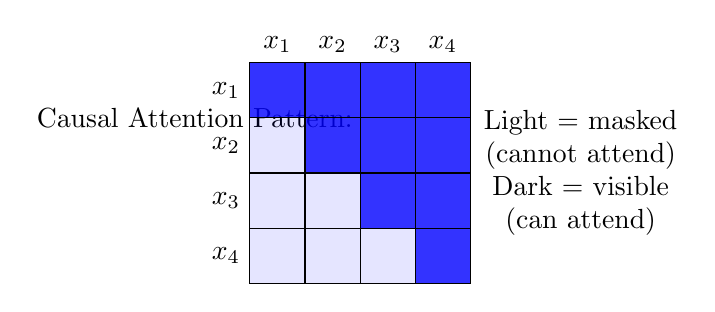
\begin{tikzpicture}[scale=0.7]
% Attention matrix
\node at (-1, 3) {Causal Attention Pattern:};

\foreach \x in {0,1,2,3} {
   \foreach \y in {0,1,2,3} {
      \pgfmathsetmacro{\opacity}{ifthenelse(\y>\x, 0.1, 0.8)}
      \fill[blue, opacity=\opacity] (\x, 3-\y) rectangle (\x+1, 4-\y);
      \draw (\x, 3-\y) rectangle (\x+1, 4-\y);
   }
}

% Labels
\node[left] at (0, 3.5) {$x_1$};
\node[left] at (0, 2.5) {$x_2$};
\node[left] at (0, 1.5) {$x_3$};
\node[left] at (0, 0.5) {$x_4$};

\node[above] at (0.5, 4) {$x_1$};
\node[above] at (1.5, 4) {$x_2$};
\node[above] at (2.5, 4) {$x_3$};
\node[above] at (3.5, 4) {$x_4$};

\node[align=center] at (6, 2) {Light = masked\\(cannot attend)\\Dark = visible\\(can attend)};
\end{tikzpicture}
\end{center}

\subsubsection{The Objective: Autoregressive (AR) Language Modeling}

This is the simplest and most intuitive objective: predict the next word. It is also known as Causal Language Modeling (CLM).

\textbf{What gets corrupted?}

Nothing is explicitly corrupted! Instead, the architecture's \textbf{causal mask} naturally hides future tokens, creating the learning signal.

\begin{center}
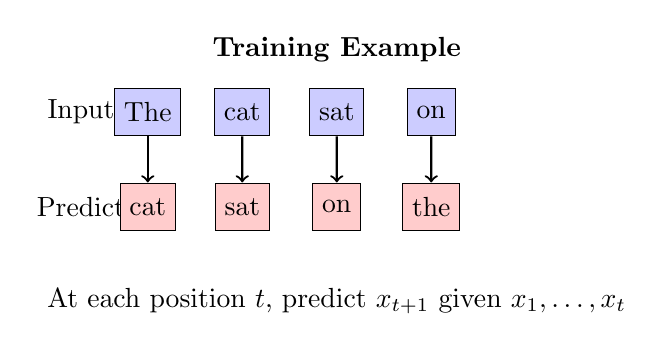
\begin{tikzpicture}[scale=0.8]
\node[align=center] at (3, 3.5) {\textbf{Training Example}};

% Input sequence
\node[align=left] at (-1, 2.5) {Input:};
\foreach \x/\word in {0/The, 1/cat, 2/sat, 3/on} {
   \node[draw, rectangle, minimum height=0.6cm, fill=blue!20] (in\x) at (\x*1.5, 2.5) {\word};
}

% Predictions
\node[align=left] at (-1, 1) {Predict:};
\foreach \x/\word in {0/cat, 1/sat, 2/on, 3/the} {
   \node[draw, rectangle, minimum height=0.6cm, fill=red!20] (pred\x) at (\x*1.5, 1) {\word};
}

% Arrows showing prediction
\foreach \x in {0,1,2,3} {
   \draw[->, thick] (in\x) -- (pred\x);
}

\node[align=center] at (3, -0.5) {At each position $t$, predict $x_{t+1}$ given $x_1, \ldots, x_t$};
\end{tikzpicture}
\end{center}

\textbf{The loss function}:
\begin{equation}
\mathcal{L}_{\text{AR}}(\theta) = -\sum_{t=1}^{T} \log p_\theta(x_t \mid x_{<t})
\end{equation}

where $x_{<t} = (x_1, \ldots, x_{t-1})$ denotes all previous tokens.

\textbf{Why it helps}:

\begin{itemize}
\item \textbf{Perfect for generation}: The training setup exactly matches inference.
\item \textbf{Teaches fluency}: Model learns grammatical structure, coherence, and natural flow.
\item \textbf{No train-test mismatch}: Uses real tokens, not artificial markers.
\end{itemize}

\textbf{Training efficiency}:

\begin{itemize}
\item \textbf{Sample efficiency}: 100\% coverage---every token contributes to the loss.
\item \textbf{Compute efficiency}: Simple, stable training; scales excellently.
\item \textbf{Parallelization}: Can compute loss for all positions simultaneously during training.
\end{itemize}

\textbf{The limitation}:

AR models only see \textit{left context}. For deep understanding tasks (classification, QA), bidirectional context is often crucial.

\textbf{Representative models}: GPT, GPT-2, GPT-3, GPT-4, LLaMA, Mistral.

\begin{tcolorbox}[colback=green!5!white, colframe=green!50!black, title=Intuition: The Storyteller]
Think of AR as training a storyteller who writes one word at a time. They see everything written so far and must predict what comes next. This makes them excellent at continuing stories, but they can't ``look ahead'' to understand the full context of a word in the middle of a sentence.
\end{tcolorbox}

\subsubsection{Scaling and In-Context Learning}

The scaling of decoder-only models led to a remarkable emergent capability: \textbf{in-context learning}.

\begin{itemize}
   \item \textbf{GPT (117M)} required fine-tuning.
   \item \textbf{GPT-2 (1.5B)} demonstrated zero-shot capabilities via prompting.
   \item \textbf{GPT-3 (175B)} showed strong few-shot learning.
\end{itemize}

Instead of fine-tuning, you provide examples directly in the prompt. No parameter updates are needed. The AR pre-training objective teaches the model to be a general-purpose pattern matcher. Given a pattern in the prompt, it continues that pattern.

\begin{verbatim}
Translate English to French:
English: Hello / French: Bonjour
English: Thank you / French: [MODEL GENERATES: "Merci"]
\end{verbatim}

\textbf{Understanding In-Context Learning: Why It Works}

Let us carefully examine why in-context learning emerges from autoregressive pre-training.

\begin{tcolorbox}[colback=green!5!white, colframe=green!50!black, title=The Mechanism Behind In-Context Learning]
During pre-training with next-token prediction on massive diverse data, the model encounters countless implicit ``tasks'' within documents:

\begin{itemize}
\item Wikipedia articles that list examples (``Common fruits include: apples, oranges, bananas...'')
\item Code with patterns (``def add(a, b): return a+b; def subtract(a, b): return a-b'')
\item Question-answer pairs in forums
\item Translation examples in language learning texts
\item Analogies and comparisons in educational content
\end{itemize}

To predict the next token accurately, the model must learn to:
\begin{enumerate}
\item \textbf{Recognize patterns} in the context
\item \textbf{Infer the implicit task} from the pattern structure
\item \textbf{Continue the pattern} appropriately
\end{enumerate}

This is precisely what in-context learning requires!
\end{tcolorbox}

\textbf{Detailed Example: How the Model Learns In-Context}

Consider this training sequence the model might encounter:

\begin{verbatim}
... In Spanish, 'hello' is 'hola', 'goodbye' is 'adiós',
and 'thank you' is 'gracias'. Similarly, in French,
'hello' is 'bonjour', 'goodbye' is 'au revoir', and ...
\end{verbatim}

When the model sees ``and'' after ``'au revoir','' it must predict the next token. To do this well, it learns:
\begin{itemize}
\item The document is showing translation examples
\item There's a pattern: English word $\rightarrow$ foreign word
\item The pattern continues for multiple examples
\item It should generate a continuation that follows this pattern
\end{itemize}

\textbf{At inference time}, when you provide:

\begin{verbatim}
Translate English to French:
sea -> mer
cat -> chat
dog ->
\end{verbatim}

The model recognizes this as the \textit{same type of pattern} it saw during training! It applies its learned pattern-continuation ability to generate ``chien''.

\textbf{The Three Modes of In-Context Learning}

\begin{enumerate}
\item \textbf{Zero-shot learning}: Task description only, no examples

\begin{verbatim}
Translate the following English word to French: hello
\end{verbatim}

The model must infer the task from the description alone. Works when the task description appeared frequently in training data.

\vspace{0.3cm}

\item \textbf{One-shot learning}: Single example provided

\begin{verbatim}
Translate English to French:
goodbye -> au revoir
hello ->
\end{verbatim}

One example clarifies the task structure. Much stronger signal than zero-shot.

\vspace{0.3cm}

\item \textbf{Few-shot learning}: Multiple examples (typically 3--10)

\begin{verbatim}
Translate English to French:
goodbye -> au revoir
thank you -> merci
good morning -> bonjour
hello ->
\end{verbatim}

Multiple examples make the pattern unmistakable. Model can learn task-specific nuances from the examples.
\end{enumerate}

\textbf{Why Does Scale Matter?}

\begin{itemize}
\item \textbf{Small models (117M)}: See patterns but can't generalize reliably. Need fine-tuning to adapt.

\item \textbf{Medium models (1.5B)}: Begin to recognize and continue simple patterns (zero-shot works for common tasks).

\item \textbf{Large models (175B+)}: Have seen so many diverse patterns during training that they can:
\begin{itemize}
\item Recognize novel task structures from examples
\item Generalize to variations they haven't seen
\item Combine multiple patterns (e.g., ``translate this metaphor'')
\end{itemize}
\end{itemize}

\begin{tcolorbox}[colback=yellow!5!white, colframe=orange!50!black, title=Why In-Context Learning is Remarkable]
Traditional view: To perform a new task, you must update the model's parameters (fine-tuning).

In-context learning: The model performs new tasks by \textit{recognizing them as instances of patterns it learned to continue during pre-training}.

\textbf{Analogy}: Like a human who, after reading thousands of books with various patterns, can recognize and continue a new pattern type (e.g., a haiku structure) without explicit training on that specific format.

\textbf{Key insight}: The pre-training objective (predict next token) implicitly teaches \textit{meta-learning}---learning to learn from context.
\end{tcolorbox}

\textbf{The Connection to Transfer Learning}

In-context learning is actually a form of \textbf{zero-parameter transfer learning}:

\begin{center}
\begin{tabular}{p{5cm}p{5cm}}
\toprule
\textbf{Traditional Transfer Learning} & \textbf{In-Context Learning} \\
\midrule
Pre-train on general data & Pre-train on general data \\
\midrule
Fine-tune parameters on task data & Provide task examples in prompt \\
\midrule
Parameters change & Parameters frozen \\
\midrule
Requires gradient updates & No gradient updates \\
\midrule
Need labeled task data & Task examples in prompt \\
\midrule
Specialized model per task & One model for all tasks \\
\bottomrule
\end{tabular}
\end{center}

\textbf{Why this matters}: In-context learning is the ultimate form of transfer learning---the model is so general that it can adapt to new tasks at inference time, with no retraining!

\subsection{Encoder-Only Architectures and Bidirectional Understanding}

\subsubsection{Architecture: Bidirectional Encoding}

Encoder-only models (like BERT, RoBERTa, ELECTRA) use \textit{only} the Transformer encoder stack.

\begin{itemize}
\item \textbf{Bidirectional self-attention}: Every token attends to all tokens (past and future).
\item \textbf{No causal mask}: The attention pattern is fully connected.
\item \textbf{Output}: Contextualized representations for each input token, ideal for classification, NER, and retrieval.
\end{itemize}

\begin{center}
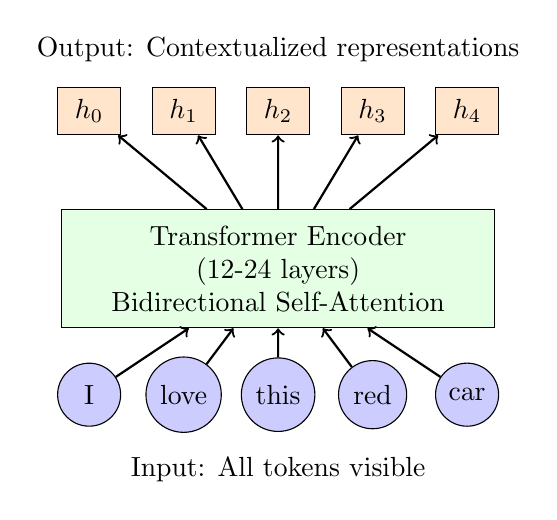
\begin{tikzpicture}[scale=0.8]
% Input tokens
\foreach \x/\word in {0/I, 1/love, 2/this, 3/red, 4/car} {
   \node[draw, circle, minimum size=0.8cm, fill=blue!20] (in\x) at (\x*1.5, 0) {\word};
}

% Encoder layers (stack of 12)
\node[draw, rectangle, minimum width=5.5cm, minimum height=1.5cm, fill=green!10] (encoder) at (3, 2) {};
\node[align=center] at (3, 2) {Transformer Encoder\\(12-24 layers)\\Bidirectional Self-Attention};

% Output representations
\foreach \x in {0,1,2,3,4} {
   \node[draw, rectangle, minimum width=0.8cm, minimum height=0.6cm, fill=orange!20] (out\x) at (\x*1.5, 4.5) {$h_{\x}$};
}

% Connections
\foreach \x in {0,1,2,3,4} {
   \draw[->, thick] (in\x) -- (encoder);
   \draw[->, thick] (encoder) -- (out\x);
}

\node[align=center, below=0.2cm of in2] {Input: All tokens visible};
\node[align=center, above=0.2cm of out2] {Output: Contextualized representations};
\end{tikzpicture}
\end{center}

Since the architecture allows bidirectional attention, we cannot use the standard AR objective (the model would just look ahead). We need objectives that leverage this bidirectionality.

\subsubsection{Objective 1: Masked Language Modeling (MLM)}

MLM (popularized by BERT) is the classic approach: hide some words and predict them using \textit{both} left and right context.

\textbf{What gets corrupted?}

\begin{enumerate}
\item Randomly select 15\% of token positions.
\item For each selected position:
\begin{itemize}
\item 80\% of the time: Replace with [MASK]
\item 10\% of the time: Replace with a random token
\item 10\% of the time: Keep unchanged
\end{itemize}
\end{enumerate}

\begin{center}
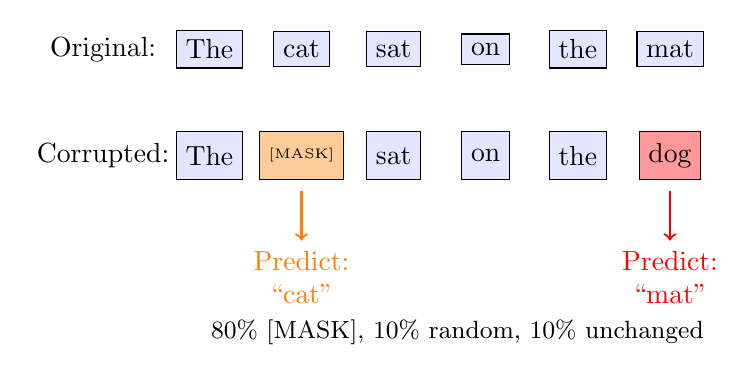
\begin{tikzpicture}[scale=0.9]
% Original
\node[align=left] at (-1.5, 3) {Original:};
\foreach \x/\word in {0/The, 1/cat, 2/sat, 3/on, 4/the, 5/mat} {
   \node[draw, rectangle, minimum height=0.3cm, fill=blue!10] at (\x*1.3, 3) {\word};
}

% Corrupted (15% = positions 1,5)
\node[align=left] at (-1.5, 1.5) {Corrupted:};
\node[draw, rectangle, minimum height=0.6cm, fill=blue!10] at (0, 1.5) {The};
\node[draw, rectangle, minimum height=0.6cm, fill=orange!40] at (1.3, 1.5) {\tiny{[MASK]}};
\node[draw, rectangle, minimum height=0.6cm, fill=blue!10] at (2.6, 1.5) {sat};
\node[draw, rectangle, minimum height=0.6cm, fill=blue!10] at (3.9, 1.5) {on};
\node[draw, rectangle, minimum height=0.6cm, fill=blue!10] at (5.2, 1.5) {the};
\node[draw, rectangle, minimum height=0.6cm, fill=red!40] at (6.5, 1.5) {dog};

% Annotations
\draw[->, thick, orange] (1.3, 1) -- (1.3, 0.3) node[below, align=center] {Predict:\\``cat''};
\draw[->, thick, red] (6.5, 1) -- (6.5, 0.3) node[below, align=center] {Predict:\\``mat''};

\node[align=center] at (3.5, -1) {\small 80\% [MASK], 10\% random, 10\% unchanged};
\end{tikzpicture}
\end{center}

\textbf{The loss function}:
\begin{equation}
\mathcal{L}_{\text{MLM}}(\theta) = -\sum_{i \in \mathcal{M}} \log p_\theta(x_i \mid x_{\setminus \mathcal{M}})
\end{equation}

where $\mathcal{M}$ is the set of masked positions.

\textbf{Why the 80/10/10 split?} It reduces the \textbf{train-test mismatch}. The [MASK] token appears during pre-training but not fine-tuning. The 10\% random/unchanged forces the model to learn representations for real tokens too.

\textbf{Why it helps}:

\begin{itemize}
\item \textbf{Bidirectional context}: The model sees both left and right context to make the prediction.
\item \textbf{Deep understanding}: Forces the model to understand relationships, not just left-to-right flow.
\end{itemize}

\textbf{Training efficiency}:

\begin{itemize}
\item \textbf{Sample efficiency}: Low! Only 15\% of tokens contribute to loss (vs. 100\% for AR). Requires 6-7$\times$ more training time to converge.
\end{itemize}

\textbf{Representative models}: BERT, RoBERTa, ALBERT, DeBERTa, DistilBERT.

\begin{tcolorbox}[colback=yellow!5!white, colframe=orange!50!black, title=Intuition: The Fill-in-the-Blank Test]
MLM is like a cloze test in school: ``The \_\_\_ sat on the mat.'' To fill in the blank, you need to understand the \textit{entire} sentence. This forces deeper understanding than just predicting the next word.
\end{tcolorbox}

\subsubsection{MLM Refinements: RoBERTa, Spans, and Whole Words}

MLM can be improved through better training procedures and structured corruption.

\textbf{RoBERTa: MLM Done Right}
RoBERTa showed that engineering improvements are crucial:
\begin{itemize}
\item \textbf{Dynamic masking}: New masks each epoch (vs. static).
\item \textbf{Remove NSP}: Next Sentence Prediction (an auxiliary task in BERT) was found to be unhelpful.
\item \textbf{Larger batches and more data} (160GB text, 500K steps).
\end{itemize}

\textbf{Span and Whole-Word Masking (WWM)}
MLM masks individual tokens, but language is structured. We can improve MLM by masking contiguous units (SpanBERT, BERT-WWM, ERNIE).

\textbf{What gets corrupted?}

Mask contiguous sequences (spans) or all subword tokens of a whole word.

\begin{center}
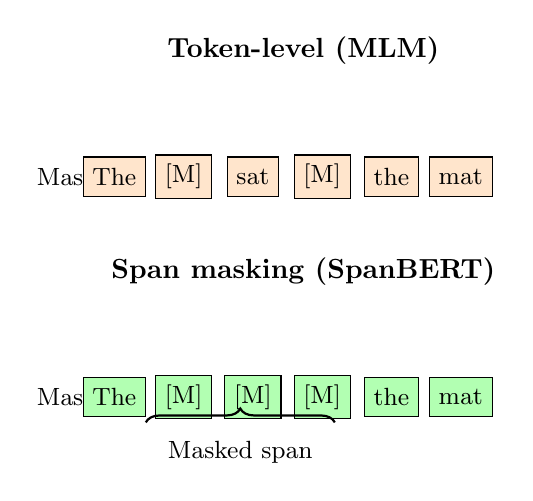
\begin{tikzpicture}[scale=0.8]
% Token-level masking
\node[align=center] at (3, 3.5) {\textbf{Token-level (MLM)}};
\node[align=left] at (-0.5, 1.5) {\small Masked:};
\foreach \x/\word in {0/The, 1/[M], 2/sat, 3/[M], 4/the, 5/mat} {
   \node[draw, rectangle, minimum height=0.5cm, fill=orange!20, font=\small] at (\x*1.1, 1.5) {\word};
}

% Span masking
\node[align=center] at (3, 0) {\textbf{Span masking (SpanBERT)}};
\node[align=left] at (-0.5, -2) {\small Masked:};
\foreach \x/\word in {0/The, 1/[M], 2/[M], 3/[M], 4/the, 5/mat} {
   \node[draw, rectangle, minimum height=0.5cm, fill=green!30, font=\small] at (\x*1.1, -2) {\word};
}

\draw[decorate, decoration={brace, amplitude=5pt}, thick] (0.5, -2.4) -- (3.5, -2.4) node[midway, below=3pt] {\small Masked span};
\end{tikzpicture}
\end{center}

\textbf{Why it helps}: Forces phrase-level understanding and is better for span-based tasks like QA and NER. SpanBERT also adds a \textbf{Span Boundary Objective (SBO)} to improve learning at the edges of the span.

\subsubsection{Objective 2: Replaced Token Detection (RTD)}

MLM is inefficient due to its 15\% coverage. Replaced Token Detection (RTD), popularized by ELECTRA, offers a more efficient alternative by changing the task from generation (predicting the token) to discrimination (detecting real vs. fake).

\textbf{What gets corrupted?}

\begin{enumerate}
\item Train a small \textbf{generator} (MLM-style) to replace $\sim$15\% of tokens with plausible alternatives.
\item A \textbf{discriminator} (the main encoder model) predicts at \textit{every} position: real or replaced?
\end{enumerate}

\begin{center}
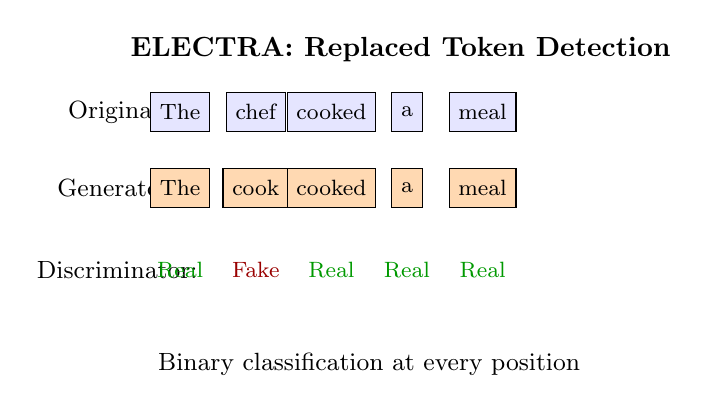
\begin{tikzpicture}[scale=0.8]
\node[align=center] at (3.5, 4) {\textbf{ELECTRA: Replaced Token Detection}};

% Original
\node[align=left] at (-1, 3) {\small Original:};
\foreach \x/\word in {0/The, 1/chef, 2/cooked, 3/a, 4/meal} {
   \node[draw, rectangle, minimum height=0.5cm, fill=blue!10, font=\footnotesize] at (\x*1.2, 3) {\word};
}

% Generator replaces "chef" with "cook"
\node[align=left] at (-1, 1.8) {\small Generator:};
\foreach \x/\word in {0/The, 1/cook, 2/cooked, 3/a, 4/meal} {
   \node[draw, rectangle, minimum height=0.5cm, fill=orange!30, font=\footnotesize] at (\x*1.2, 1.8) {\word};
}

% Discriminator labels
\node[align=left] at (-1, 0.5) {\small Discriminator:};
\node[font=\footnotesize, green!60!black] at (0, 0.5) {Real};
\node[font=\footnotesize, red!60!black] at (1.2, 0.5) {Fake};
\node[font=\footnotesize, green!60!black] at (2.4, 0.5) {Real};
\node[font=\footnotesize, green!60!black] at (3.6, 0.5) {Real};
\node[font=\footnotesize, green!60!black] at (4.8, 0.5) {Real};

\node[align=center, font=\small] at (3, -1) {Binary classification at every position};
\end{tikzpicture}
\end{center}

\textbf{The loss function} (Discriminator):
\begin{equation}
\mathcal{L}_D(\theta_D) = -\sum_{t=1}^{T} \left[ \mathbf{1}_{x_t = \tilde{x}_t} \log D(x_t, t) + \mathbf{1}_{x_t \neq \tilde{x}_t} \log (1 - D(x_t, t)) \right]
\end{equation}
where $D(x_t, t)$ is the probability that token $t$ is real. The generator is discarded after pre-training.

\textbf{Why it helps}:

\begin{itemize}
\item \textbf{100\% sample efficiency}: Every token contributes to the loss.
\item \textbf{No [MASK] tokens}: Uses natural text, reducing train-test mismatch.
\item \textbf{Compute efficient}: Binary classification is cheaper than vocabulary softmax. ELECTRA-Small matches BERT-Base performance with 1/4 the compute.
\end{itemize}

\textbf{Representative models}: ELECTRA, DeBERTa-v3 (hybrid).

\begin{tcolorbox}[colback=yellow!5!white, colframe=orange!50!black, title=Intuition: The Forgery Detector]
RTD is like training an art forgery detector. A forger (generator) creates plausible fakes. Your job (discriminator) is to examine \textit{every brushstroke} and determine if it's original or fake. Detecting whether ``cook'' or ``chef'' is correct requires deep understanding, but is computationally cheaper than MLM.
\end{tcolorbox}

\subsubsection{Fine-tuning Encoders}

After pre-training, encoders are adapted by adding task-specific heads, and the entire model is typically updated during fine-tuning.

\begin{itemize}
\item \textbf{Classification} (e.g., sentiment): Use the [CLS] token representation + classification head.
\item \textbf{Token-level tasks (NER)}: Use representation of each token + token classifier.
\item \textbf{Sentence pair tasks (NLI)}: Input: [CLS] Premise [SEP] Hypothesis [SEP]; use [CLS] representation.
\end{itemize}

\begin{center}
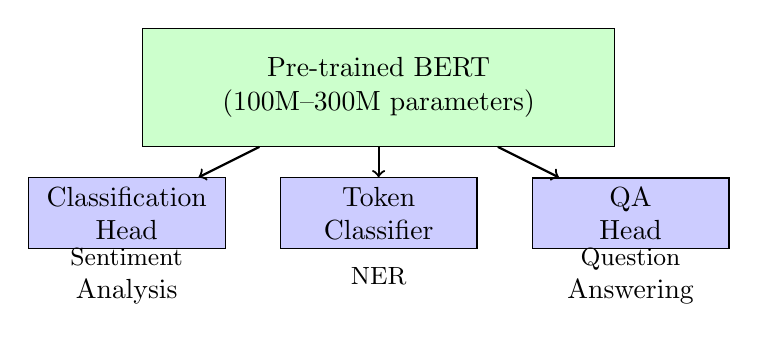
\begin{tikzpicture}[scale=0.8]
% Pre-trained BERT
\node[draw, rectangle, minimum width=6cm, minimum height=1.5cm, fill=green!20, align = center] (bert) at (0,0)
   {Pre-trained BERT\\(100M--300M parameters)};

% Task-specific heads
\node[draw, rectangle, minimum width=2.5cm, minimum height=0.8cm, fill=blue!20, align = center] (cls) at (-4,-2)
   {Classification\\Head};
\node[draw, rectangle, minimum width=2.5cm, minimum height=0.8cm, fill=blue!20, align = center] (tok) at (0,-2)
   {Token\\Classifier};
\node[draw, rectangle, minimum width=2.5cm, minimum height=0.8cm, fill=blue!20, align = center] (qa) at (4,-2)
   {QA\\Head};

\draw[->, thick] (bert) -- (cls);
\draw[->, thick] (bert) -- (tok);
\draw[->, thick] (bert) -- (qa);

\node[align=center, align = center] at (-4, -3) {\small Sentiment\\Analysis};
\node[align=center] at (0, -3) {\small NER};
\node[align=center, align = center] at (4, -3) {\small Question\\Answering};
\end{tikzpicture}
\end{center}

\subsection{Encoder-Decoder Architectures and Denoising Autoencoding}

\subsubsection{Architecture: Sequence-to-Sequence}

Encoder-Decoder models (like T5, BART) use the \textit{full} Transformer architecture.

\begin{itemize}
\item \textbf{Encoder}: Bidirectional self-attention (like BERT) to understand the input.
\item \textbf{Decoder}: Causal self-attention (like GPT) to generate the output.
\item \textbf{Cross-Attention}: The decoder attends to the encoder's output.
\item \textbf{Best for}: Tasks where input is consumed and output is generated (translation, summarization).
\end{itemize}

T5 (Text-to-Text Transfer Transformer) popularized the \textbf{Text-to-Text Framework}, where every task is framed as input text generating output text.

\begin{center}
\begin{tabular}{ll}
\toprule
\textbf{Task} & \textbf{Format} \\
\midrule
Translation & Input: ``translate English to German: Hello'' $\rightarrow$ Output: ``Hallo'' \\
Classification & Input: ``sentiment: I love this movie'' $\rightarrow$ Output: ``positive'' \\
\bottomrule
\end{tabular}
\end{center}

\subsubsection{The Objective: Denoising Autoencoding (DAE)}

The solution: corrupt the input (encoder side), then generate the clean output (decoder side).

\textbf{The general framework}:
\begin{equation}
\mathcal{L}_{\text{DAE}}(\theta) = -\mathbb{E}_{x} \mathbb{E}_{\tilde{x} \sim q(\cdot \mid x)} \log p_\theta(x \mid \tilde{x})
\end{equation}
where $q(\tilde{x} \mid x)$ is a corruption distribution.

\subsubsection{DAE Variant 1: T5 Span Corruption}

T5 adapts span masking for the seq2seq setting.

\textbf{What gets corrupted?}

\begin{enumerate}
\item Mask random spans (average length 3 tokens, 15\% of tokens total).
\item Replace each masked span with a unique sentinel token ($\langle X \rangle$, $\langle Y \rangle$, etc.).
\item Encoder sees corrupted text; decoder generates the original spans indicated by the sentinels.
\end{enumerate}

\begin{center}
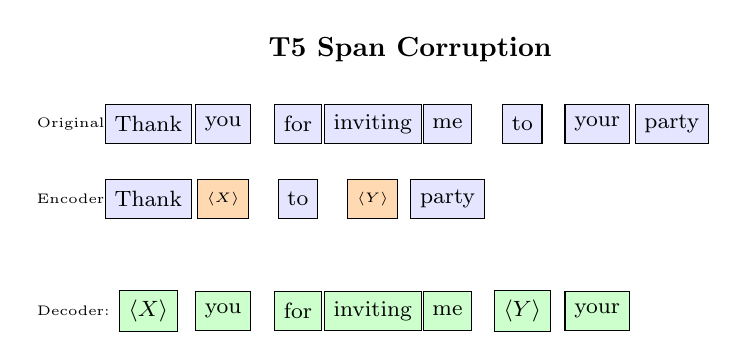
\begin{tikzpicture}[scale=0.95]
\node[align=center] at (3.5, 4) {\textbf{T5 Span Corruption}};

% Original
\node[align=left] at (-1, 3) {\tiny Original:};
\foreach \x/\word in {0/Thank, 1/you, 2/for, 3/inviting, 4/me, 5/to, 6/your, 7/party} {
   \node[draw, rectangle, minimum height=0.5cm, fill=blue!10, font=\footnotesize] at (\x*1, 3) {\word};
}

% Encoder input
\node[align=left] at (-1, 2) {\tiny Encoder:};
\node[draw, rectangle, minimum height=0.5cm, fill=blue!10, font=\footnotesize] at (0, 2) {Thank};
\node[draw, rectangle, minimum height=0.5cm, fill=orange!30, font=\footnotesize] at (1, 2) {\tiny{$\langle X \rangle$}};
\node[draw, rectangle, minimum height=0.5cm, fill=blue!10, font=\footnotesize] at (2, 2) {to};
\node[draw, rectangle, minimum height=0.5cm, fill=orange!30, font=\footnotesize] at (3, 2) {\tiny{$\langle Y \rangle$}};
\node[draw, rectangle, minimum height=0.5cm, fill=blue!10, font=\footnotesize] at (4, 2) {party};

% Decoder target
\node[align=left] at (-1, 0.5) {\tiny Decoder:};
\node[draw, rectangle, minimum height=0.5cm, fill=green!20, font=\footnotesize] at (0, 0.5) {$\langle X \rangle$};
\node[draw, rectangle, minimum height=0.5cm, fill=green!20, font=\footnotesize] at (1, 0.5) {you};
\node[draw, rectangle, minimum height=0.5cm, fill=green!20, font=\footnotesize] at (2, 0.5) {for};
\node[draw, rectangle, minimum height=0.5cm, fill=green!20, font=\footnotesize] at (3, 0.5) {inviting};
\node[draw, rectangle, minimum height=0.5cm, fill=green!20, font=\footnotesize] at (4, 0.5) {me};
\node[draw, rectangle, minimum height=0.5cm, fill=green!20, font=\footnotesize] at (5, 0.5) {$\langle Y \rangle$};
\node[draw, rectangle, minimum height=0.5cm, fill=green!20, font=\footnotesize] at (6, 0.5) {your};
\end{tikzpicture}
\end{center}

\textbf{Why it helps}:

\begin{itemize}
\item \textbf{Encoder learns compression/understanding}; \textbf{Decoder learns generation}.
\item \textbf{High sample efficiency}: Decoder loss is calculated on all generated tokens (100\% coverage on targets).
\end{itemize}

\textbf{Representative models}: T5, UL2.

\subsubsection{DAE Variant 2: BART Diverse Noise}

BART uses a \textit{mixture} of corruption strategies, forcing the model to reconstruct the fully clean original text.

\begin{itemize}
\item \textbf{Text infilling}: Replace spans with single [MASK].
\item \textbf{Sentence permutation}: Shuffle sentence order.
\item \textbf{Token deletion/masking/rotation}.
\end{itemize}

\textbf{Why it helps}: Exposure to diverse noise teaches robust representations, particularly strong for abstractive summarization and paraphrasing.

\textbf{Representative models}: BART, mBART (multilingual).

\begin{tcolorbox}[colback=green!5!white, colframe=green!50!black, title=Intuition: The Document Repair Shop]
Think of DAE objectives like a document restoration service. You're given damaged texts (missing words, shuffled sentences) and must reconstruct the pristine original. This teaches both understanding (what's wrong?) and generation (how to fix it?).
\end{tcolorbox}

\subsection{Advanced and Hybrid Objectives}

\subsubsection{Permutation Language Modeling (PLM)}

Can we get bidirectional context \textit{without} using artificial [MASK] tokens and without a full encoder-decoder setup? Yes, via permutation (XLNet).

\textbf{What gets corrupted?}

We corrupt the \textit{order}, not the tokens.

\begin{enumerate}
\item Sample a random permutation $z$ of the sequence positions $[1, 2, \ldots, T]$.
\item Predict each token in the order given by $z$, using previous tokens in that permutation (Autoregressive factorization).
\end{enumerate}

\textbf{Example}: Original: ``The cat sat''. Permutation $z = [2, 1, 3]$:
\begin{itemize}
\item Predict $x_2$ (``cat'') first (no context).
\item Then predict $x_1$ (``The'') given $x_2$ (``cat'').
\item Finally predict $x_3$ (``sat'') given $x_1, x_2$ (``The cat'').
\end{itemize}

\textbf{The loss function}:
\begin{equation}
\mathcal{L}_{\text{PLM}}(\theta) = -\mathbb{E}_{z} \sum_{t=1}^{T} \log p_\theta(x_{z_t} \mid x_{z_{<t}})
\end{equation}

\textbf{Why it helps}:

\begin{itemize}
\item \textbf{Bidirectional context}: In expectation, each token sees all others as context.
\item \textbf{No [MASK] tokens} and \textbf{100\% sample efficiency}.
\end{itemize}

\textbf{The limitation}: Implementation is complex (requires two-stream self-attention) and computationally expensive.

\begin{tcolorbox}[colback=yellow!5!white, colframe=orange!50!black, title=Intuition: The Shuffled Deck]
Imagine reading a shuffled sentence where words appear in random order, but you can see all previous words. Sometimes you see the end before the beginning! This teaches you to understand words in context from \textit{any} direction, not just left-to-right.
\end{tcolorbox}

\subsubsection{UL2: Mixture of Denoisers}

UL2 (Unified Language Learner) trains a single model (typically encoder-decoder) on a mixture of objectives:

\begin{enumerate}
\item \textbf{R-denoiser}: Regular span corruption (like T5).
\item \textbf{S-denoiser}: Short, aggressive corruption (extreme masking).
\item \textbf{X-denoiser}: Long-range dependencies (large spans, document-level).
\end{enumerate}

\textbf{Mode switching}: Uses special tokens (<R>, <S>, $\langle X \rangle$) to indicate the denoising mode, allowing the model to adapt its behavior. Results in strong performance on both generative and understanding tasks.

\subsection{Comparative Analysis and Practical Guide}

\subsubsection{Unified Mathematical Framework}

All SSL objectives can be expressed in a common form, revealing the key design dimensions: Corruption strategy, Loss coverage, Context structure, and Prediction target.

\begin{equation}
\min_\theta \mathbb{E}_{x \sim \mathcal{D}} \mathbb{E}_{\tilde{x} \sim q(\cdot \mid x)} \left[ -\sum_{t \in \mathcal{T}(\tilde{x})} w_t \log p_\theta(f_t(x) \mid \text{context}(\tilde{x}, t)) \right]
\end{equation}

\begin{center}
\begin{tabular}{@{}llllll@{}}
\toprule
\textbf{Obj.} & \textbf{Arch.} & \textbf{Corruption} $q$ & \textbf{Coverage} $\mathcal{T}$ & \textbf{Context} & \textbf{Target} $f_t$ \\
\midrule
AR & Decoder & Causal mask & 100\% & $x_{<t}$ & $x_t$ \\
MLM & Encoder & Random mask & $\sim$15\% & $x_{\setminus \mathcal{M}}$ & $x_t$ \\
RTD & Encoder & Plausible replace & 100\% & $\tilde{x}$ & Real/Fake \\
PLM & Hybrid & Permutation & 100\% & $x_{z_{<t}}$ & $x_{z_t}$ \\
T5 & Enc-Dec & Span $\rightarrow$ sentinel & 100\% (decoder) & Enc + prev & $x_t$ \\
\bottomrule
\end{tabular}
\end{center}

\subsubsection{Efficiency Comparison}

Efficiency is crucial for scaling.

\begin{center}
\begin{tabular}{@{}lllcccl@{}}
\toprule
\textbf{Obj.} & \textbf{Arch.} & \textbf{Coverage} & \textbf{Bidir?} & \textbf{Mismatch} & \textbf{Efficiency} & \textbf{Best For} \\
\midrule
AR & Decoder & 100\% & No & None & $\bigstar\bigstar\bigstar\bigstar$ & Generation \\
MLM & Encoder & 15\% & Yes & [MASK] & $\bigstar\bigstar$ & Understanding \\
Span & Encoder & 15\% & Yes & [MASK] & $\bigstar\bigstar$ & Span tasks \\
RTD & Encoder & 100\% & Yes & Minimal & $\bigstar\bigstar\bigstar\bigstar\bigstar$ & Efficient Encoders \\
PLM & Hybrid & 100\% & Yes & Low & $\bigstar\bigstar\bigstar$ & Hybrid (Complex) \\
DAE & Enc-Dec & 100\% & Enc: Yes & Minimal & $\bigstar\bigstar\bigstar\bigstar$ & Seq2seq \\
\bottomrule
\end{tabular}
\end{center}

\textbf{Key efficiency insights}:

\begin{enumerate}
\item \textbf{Loss coverage matters}: MLM's 15\% coverage is a major bottleneck compared to 100\% coverage objectives.
\item \textbf{RTD is the efficiency champion} for encoders (100\% coverage + cheaper binary loss).
\item \textbf{AR is the champion for scaling}: Simple objective, 100\% coverage, stable training.
\end{enumerate}

\subsubsection{Practical Decision Guide}

\begin{tcolorbox}[colback=blue!5!white, colframe=blue!75!black, title=Decision Tree: Choosing Architecture and Objective]
\textbf{Step 1}: Do you need to generate variable-length text?
\begin{itemize}
\item No (classification, tagging, retrieval) $\rightarrow$ Go to Step 2 (Encoder-only)
\item Yes (generation, translation, summarization) $\rightarrow$ Go to Step 3 (Decoder or Enc-Dec)
\end{itemize}

\textbf{Step 2}: Encoder-only tasks
\begin{itemize}
\item Limited compute or need maximum efficiency? $\rightarrow$ \textbf{RTD (ELECTRA/DeBERTa-v3)}
\item Standard budget, focus on performance? $\rightarrow$ \textbf{MLM (RoBERTa)}
\item Span-focused tasks (QA, NER)? $\rightarrow$ \textbf{Span masking (SpanBERT)}
\end{itemize}

\textbf{Step 3}: Generation tasks
\begin{itemize}
\item Conditional generation (input-heavy: translation, summarization)? $\rightarrow$ \textbf{Enc-Dec with DAE (T5, BART)}
\item Open-ended generation (chat, completion, few-shot)? $\rightarrow$ \textbf{Decoder-only with AR (GPT, LLaMA)}
\item Want a single model for both understanding and generation? $\rightarrow$ \textbf{Enc-Dec with Mixture (UL2, Flan-T5) or Large Decoder-Only}
\end{itemize}
\end{tcolorbox}

\subsection{Emerging Trends and Future Directions}

\subsubsection{Scaling Beyond Pre-training Objectives}

Recent work shows that \textit{how} you scale and what you do \textit{after} pre-training matters as much as the objective itself:

\begin{itemize}
\item \textbf{Instruction tuning} (Flan, InstructGPT): Aligning the model with human tasks after pre-training often has a larger impact than the initial objective.
\item \textbf{Mixture of experts (MoE)}: Efficiently scaling parameters by activating only parts of the model per token (Switch Transformers, GLaM, Mixtral).
\item \textbf{Retrieval augmentation}: Combine pre-training with external knowledge retrieval (RETRO, Atlas).
\end{itemize}

\subsubsection{Unified Objectives and Architectures}

The trend is toward unification, blurring the lines between the families:

\begin{itemize}
\item \textbf{Prefix LM} (e.g., PaLM, BLOOM): A modification to decoder-only models allowing bidirectional attention on a prefix (input) and causal attention on the generated output. This gives decoder-only models encoder-like capabilities.
\item \textbf{Dominance of Decoder-Only}: Due to their simplicity, scalability, and emergent in-context learning abilities, decoder-only models trained with the AR objective are currently the dominant paradigm in large-scale NLP.
\end{itemize}

\section{Key Takeaways}

\begin{tcolorbox}[colback=green!5!white, colframe=green!50!black, title=Core Principles: Transfer Learning and Self-Supervision]

\textbf{The Universal Principle: Transfer Learning}

Transfer learning is the fundamental paradigm behind modern deep learning:
\begin{enumerate}
\item \textbf{Pre-train} on large, general-purpose data to learn universal features
\item \textbf{Adapt} to specific tasks with much smaller datasets
\item The general features learned in stage 1 transfer to stage 2
\end{enumerate}

This works across modalities---vision, language, speech, multimodal---because deep hierarchical representations have transferable structure.

\vspace{0.3cm}

\textbf{The NLP Innovation: Self-Supervision}

NLP's breakthrough was realizing you don't need labeled data for pre-training:
\begin{itemize}
\item Computer vision: Needed ImageNet (millions of human-labeled images)
\item NLP: Uses self-supervision (text provides its own labels)
\item Result: Unlimited pre-training data from the entire internet!
\end{itemize}

This made NLP models more powerful than CV models initially, because:
\begin{enumerate}
\item More pre-training data (trillions vs. millions)
\item Data is free (no annotation cost)
\item Easy to scale (just scrape more text)
\end{enumerate}

\vspace{0.3cm}

\textbf{Why It Took Time: The Discrete vs. Continuous Challenge}

\begin{itemize}
\item Text has discrete tokens ($\sim$50K vocabulary) $\rightarrow$ natural prediction task
\item Images have ``infinite vocabulary'' (continuous pixels) $\rightarrow$ needed different SSL approaches
\item Text SSL breakthrough (2018) inspired vision SSL (2020+: SimCLR, MAE, etc.)
\end{itemize}
\end{tcolorbox}

\begin{tcolorbox}[colback=green!5!white, colframe=green!50!black, title=Core Principles of SSL Objectives]
\begin{enumerate}
\item \textbf{There's no one-size-fits-all objective}
\begin{itemize}
\item AR for generation, MLM/RTD for understanding, DAE for seq2seq
\end{itemize}

\item \textbf{Efficiency has multiple dimensions}
\begin{itemize}
\item Sample efficiency (loss coverage): 15\% vs. 100\%
\item Compute efficiency: Binary loss vs. vocabulary softmax
\item Scaling efficiency: Stability, parallelization
\end{itemize}

\item \textbf{Train-test mismatch matters, but can be managed}
\begin{itemize}
\item [MASK] tokens are the main culprit
\item 80/10/10 split, RTD, and PLM all address this
\end{itemize}

\item \textbf{Bidirectionality vs. causality is the fundamental trade-off}
\begin{itemize}
\item Understanding needs bidirectional context
\item Generation needs causal structure
\item Encoder-decoder architectures get both
\end{itemize}

\item \textbf{Engineering details matter enormously}
\begin{itemize}
\item RoBERTa: same architecture, better training = huge gains
\item Dynamic masking, batch size, training length all critical
\end{itemize}

\item \textbf{The field is converging on flexible, unified approaches}
\begin{itemize}
\item Mixture objectives (UL2)
\item Instruction tuning after pre-training
\item In-context learning reduces objective importance
\end{itemize}

\item \textbf{Scale enables qualitative changes}
\begin{itemize}
\item Small models: Need fine-tuning
\item Medium models: Zero-shot for simple tasks
\item Large models: Few-shot learning, in-context adaptation
\item This is transfer learning evolving beyond parameter updates!
\end{itemize}
\end{enumerate}
\end{tcolorbox}

\subsection{Practical Implementation Tips}

\begin{enumerate}
\item \textbf{Start simple}: Begin with AR (for decoders) or MLM (for encoders) before trying exotic objectives

\item \textbf{Match objective to architecture}:
\begin{itemize}
\item Encoder-only $\rightarrow$ MLM or RTD
\item Decoder-only $\rightarrow$ AR
\item Encoder-decoder $\rightarrow$ DAE (T5, BART)
\end{itemize}

\item \textbf{For MLM, use RoBERTa improvements}:
\begin{itemize}
\item Dynamic masking (regenerate masks each epoch)
\item Large batches (as large as your memory allows)
\item Remove NSP (doesn't help)
\end{itemize}

\item \textbf{For limited compute, use RTD}:
\begin{itemize}
\item ELECTRA-Small matches BERT-Base with 1/4 compute
\item Use a small generator (1/4 to 1/3 discriminator size)
\end{itemize}

\item \textbf{For seq2seq, prefer T5-style span corruption}:
\begin{itemize}
\item Simpler than BART's mixture
\item Stable training
\item Works well at scale
\end{itemize}

\item \textbf{Monitor train-test alignment}:
\begin{itemize}
\item If pre-training uses [MASK], test with and without
\item If using PLM or RTD, verify no information leakage
\end{itemize}

\item \textbf{Ablate carefully}:
\begin{itemize}
\item Masking ratio (10-20\% range)
\item Span length (geometric distribution, mean 3-5)
\item For RTD, generator size (1/4 to 1/2 discriminator)
\end{itemize}
\end{enumerate}

\section{Homework Assignment}

\subsection{Conceptual Questions}

\begin{enumerate}
\item \textbf{Transfer Learning Analogy}:
\begin{itemize}
\item Explain the parallel between ImageNet pre-training in computer vision and masked language modeling in NLP. What are the corresponding stages, and what gets transferred in each case?
\item What are the key differences? Why is NLP's self-supervised approach actually \textit{more powerful} than CV's supervised ImageNet approach?
\item Why did text SSL come before vision SSL, even though CV had transfer learning first?
\end{itemize}

\item \textbf{Self-Supervision Across Modalities}:
\begin{itemize}
\item Explain why predicting masked words is a natural SSL task for text, but predicting individual pixels is not effective for images.
\item Research and explain how modern vision SSL methods (SimCLR or MAE) work around the ``infinite vocabulary'' problem.
\item What does this tell us about designing SSL objectives in general?
\end{itemize}

\item \textbf{In-Context Learning}:
\begin{itemize}
\item Explain mechanistically why autoregressive pre-training leads to in-context learning ability. What implicit ``meta-learning'' happens during pre-training?
\item Why does in-context learning only emerge at scale (GPT-3, 175B) but not in smaller models (GPT, 117M)?
\item Compare in-context learning to traditional transfer learning. How is providing examples in a prompt similar to, and different from, fine-tuning?
\end{itemize}

\item \textbf{Objective Comparison}:
\begin{itemize}
\item Calculate how many training steps are needed for MLM vs. AR to see each token as a prediction target, assuming 15\% masking rate for MLM
\item If AR takes 100K steps to converge, estimate steps needed for MLM
\item Why might MLM still be worth using despite lower sample efficiency?
\end{itemize}

\item \textbf{Understanding RTD}:
\begin{itemize}
\item Why does RTD use a \textit{plausible} generator rather than random token replacement?
\item What would happen if the generator was too good? Too bad?
\item Why is binary classification cheaper than vocabulary softmax, and how much faster is it?
\end{itemize}
\end{enumerate}

\subsection{Design Exercise}

\textbf{Design Your Own Objective}:
\begin{itemize}
\item Design an SSL objective for code (Python/Java)
\item What should you corrupt? Why?
\item Would standard MLM work well? Why or why not?
\item Justify your design choices
\end{itemize}

\subsection{Efficiency Analysis}

\begin{enumerate}
\item Given a sequence of length 512:
\begin{itemize}
\item How many tokens contribute to AR loss?
\item How many for MLM (15\% masking)?
\item How many for RTD?
\end{itemize}

\item Why does RTD's binary classification make it faster despite 100\% coverage?

\item Compare the computational costs of:
\begin{itemize}
\item MLM with vocabulary size 30,000
\item RTD with the same vocabulary
\item Which is more efficient? By how much?
\end{itemize}
\end{enumerate}

\subsection{Implementation Challenge}

\begin{enumerate}
\item \textbf{Implement the 80/10/10 masking strategy for MLM}:
\begin{itemize}
\item Given a sentence, apply this corruption
\item Verify the percentages are correct in expectation
\item Test on multiple sentences and average the results
\end{itemize}

\item \textbf{T5 Span Corruption}:
\begin{itemize}
\item Given ``The quick brown fox jumped over the lazy dog''
\item Apply T5 span corruption with 15\% corruption rate, mean span length 3
\item Show both encoder input and decoder target with sentinels
\end{itemize}
\end{enumerate}

\subsection{Trade-off Analysis}

You have $10^{21}$ FLOPs for pre-training an encoder:
\begin{itemize}
\item Compare: (a) BERT-style MLM, (b) ELECTRA-style RTD
\item Which objective would you choose? Why?
\item How would your answer change with $10^{23}$ FLOPs?
\item Consider: sample efficiency, compute efficiency, final performance
\end{itemize}

\section{Synthesis: The Evolution of Transfer Learning}

Before we conclude, let us step back and see the bigger picture of how transfer learning has evolved.

\subsection{The Transfer Learning Paradigm Across Time}

\begin{center}
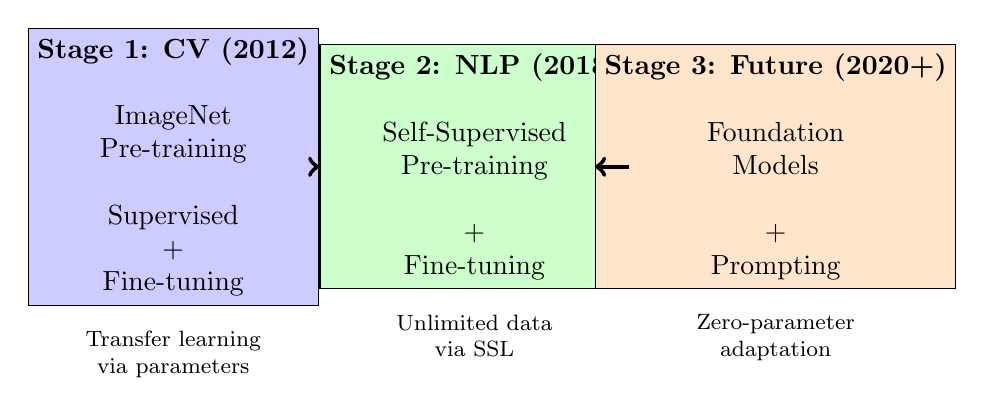
\begin{tikzpicture}[scale=0.85]
% Three stages
\node[draw, rectangle, minimum width=3.5cm, minimum height=2.5cm, fill=blue!20, align=center] (cv) at (0,0)
   {\textbf{Stage 1: CV (2012)}\\\\ImageNet\\Pre-training\\\\Supervised\\+\\Fine-tuning};

\node[draw, rectangle, minimum width=3.5cm, minimum height=2.5cm, fill=green!20, align=center] (nlp) at (4.5,0)
   {\textbf{Stage 2: NLP (2018)}\\\\Self-Supervised\\Pre-training\\\\+\\Fine-tuning};

\node[draw, rectangle, minimum width=3.5cm, minimum height=2.5cm, fill=orange!20, align=center] (icl) at (9,0)
   {\textbf{Stage 3: Future (2020+)}\\\\Foundation\\Models\\\\+\\Prompting};

\draw[->, ultra thick] (cv) -- (nlp);
\draw[->, ultra thick] (nlp) -- (icl);

\node[below=0.2cm of cv, align=center, font=\footnotesize] {Transfer learning\\via parameters};
\node[below=0.2cm of nlp, align=center, font=\footnotesize] {Unlimited data\\via SSL};
\node[below=0.2cm of icl, align=center, font=\footnotesize] {Zero-parameter\\adaptation};
\end{tikzpicture}
\end{center}

\subsection{What Changed at Each Stage?}

\begin{center}
\begin{tabular}{p{3cm}p{3.5cm}p{3.5cm}p{3.5cm}}
\toprule
\textbf{Aspect} & \textbf{CV (2012--2017)} & \textbf{NLP (2018--2020)} & \textbf{Foundation Models (2020+)} \\
\midrule
Pre-training data & ImageNet (1.2M images, labeled) & Web text (100B+ tokens, unlabeled) & Massive multimodal (text, images, code) \\
\midrule
Pre-training task & Supervised classification & Self-supervised (MLM, AR) & Self-supervised at huge scale \\
\midrule
Adaptation & Fine-tune all or freeze early layers & Fine-tune with small LR & Prompting (no parameter updates) \\
\midrule
Task data needed & 1K--10K examples & 1K--10K examples & 0--10 examples (in prompt) \\
\midrule
Compute for adaptation & Hours (fine-tuning) & Hours (fine-tuning) & Seconds (inference) \\
\midrule
Resulting model & Task-specific & Task-specific & General-purpose \\
\midrule
Key limitation & Need labeled pre-train data & Need task fine-tuning & Requires massive scale \\
\midrule
Key innovation & Feature transfer & Self-supervision & In-context learning \\
\bottomrule
\end{tabular}
\end{center}

\subsection{The Trajectory: From Specialized to General}

\begin{tcolorbox}[colback=blue!5!white, colframe=blue!75!black, title=The Progression of Generality]

\textbf{Level 1: No Transfer (Pre-2012)}
\begin{itemize}
\item Train from scratch for each task
\item Need massive labeled datasets per task
\item Limited by data availability
\end{itemize}

\vspace{0.3cm}

\textbf{Level 2: Supervised Transfer Learning (2012--2017)}
\begin{itemize}
\item Pre-train once on labeled data (ImageNet)
\item Fine-tune for each task
\item Reduces task data needs by 10--100x
\item But: Pre-training bottlenecked by labeled data
\end{itemize}

\vspace{0.3cm}

\textbf{Level 3: Self-Supervised Transfer Learning (2018--2020)}
\begin{itemize}
\item Pre-train on unlimited unlabeled data
\item Fine-tune for each task
\item Reduces task data needs by 10--100x
\item Scales better: unlimited pre-training data
\end{itemize}

\vspace{0.3cm}

\textbf{Level 4: Foundation Models with In-Context Learning (2020+)}
\begin{itemize}
\item Pre-train on massive scale (100B+ parameters, trillions of tokens)
\item No fine-tuning needed---just prompt!
\item Reduces task data needs to 0--10 examples
\item Single model for all tasks
\item \textit{This is the ultimate transfer learning: zero-parameter adaptation}
\end{itemize}
\end{tcolorbox}

\subsection{Why This Progression Makes Sense}

Each stage solved the bottleneck of the previous stage:

\begin{enumerate}
\item \textbf{Pre-2012 bottleneck}: Need huge labeled datasets per task
\begin{itemize}
\item \textbf{Solution}: Transfer learning (pre-train once, reuse features)
\end{itemize}

\item \textbf{2012--2017 bottleneck}: Pre-training limited by labeled data (ImageNet took years to create)
\begin{itemize}
\item \textbf{Solution}: Self-supervised learning (unlimited unlabeled data)
\end{itemize}

\item \textbf{2018--2020 bottleneck}: Still need fine-tuning for each task (costly, requires task data)
\begin{itemize}
\item \textbf{Solution}: Scale to enable in-context learning (no fine-tuning needed)
\end{itemize}

\item \textbf{Current bottleneck}: Massive compute for pre-training (only large organizations can do it)
\begin{itemize}
\item \textbf{Active research}: Efficient pre-training, smaller models with strong performance, parameter-efficient fine-tuning
\end{itemize}
\end{enumerate}

\subsection{The Unifying Principle}

Despite these different stages, the core principle remains the same:

\begin{tcolorbox}[colback=green!5!white, colframe=green!50!black, title=The Universal Law of Transfer Learning]
\textbf{Learn general-purpose representations from abundant data, then adapt to specific tasks with minimal task-specific data.}

What changed over time:
\begin{itemize}
\item \textbf{More abundant data}: labeled ImageNet $\rightarrow$ unlabeled internet
\item \textbf{More general representations}: visual features $\rightarrow$ linguistic + world knowledge $\rightarrow$ multimodal understanding
\item \textbf{More efficient adaptation}: fine-tuning $\rightarrow$ prompting
\end{itemize}

But the fundamental insight---that deep networks learn hierarchical, transferable representations---remains the same.
\end{tcolorbox}

\subsection{Implications for the Future}

Where is this heading?

\begin{itemize}
\item \textbf{Multimodal foundation models}: Text + images + audio + video (e.g., GPT-4, Gemini)

\item \textbf{Unified architectures}: Single model for all modalities (already happening)

\item \textbf{Continued scaling}: Models will grow, requiring distributed training

\item \textbf{Efficiency focus}: Making these capabilities accessible (distillation, quantization, efficient architectures)

\item \textbf{New adaptation modes}: Beyond prompting---what's next after zero-parameter adaptation?
\end{itemize}

The trajectory is clear: \textbf{from specialized models requiring lots of task data, to general-purpose models requiring no task data}.

\section{Further Reading}

\subsection{Foundational Papers}

\begin{itemize}
\item \textbf{BERT}: Devlin et al. (2018). ``BERT: Pre-training of Deep Bidirectional Transformers for Language Understanding.''

\item \textbf{GPT}: Radford et al. (2018). ``Improving Language Understanding by Generative Pre-Training.''

\item \textbf{GPT-2}: Radford et al. (2019). ``Language Models are Unsupervised Multitask Learners.''

\item \textbf{GPT-3}: Brown et al. (2020). ``Language Models are Few-Shot Learners.''

\item \textbf{T5}: Raffel et al. (2020). ``Exploring the Limits of Transfer Learning with a Unified Text-to-Text Transformer.''
\end{itemize}

\subsection{SSL Objectives}

\begin{itemize}
\item \textbf{RoBERTa}: Liu et al. (2019). ``RoBERTa: A Robustly Optimized BERT Pretraining Approach.''

\item \textbf{SpanBERT}: Joshi et al. (2020). ``SpanBERT: Improving Pre-training by Representing and Predicting Spans.''

\item \textbf{XLNet}: Yang et al. (2019). ``XLNet: Generalized Autoregressive Pretraining for Language Understanding.''

\item \textbf{ELECTRA}: Clark et al. (2020). ``ELECTRA: Pre-training Text Encoders as Discriminators Rather Than Generators.''

\item \textbf{BART}: Lewis et al. (2020). ``BART: Denoising Sequence-to-Sequence Pre-training for Natural Language Generation, Translation, and Comprehension.''

\item \textbf{UL2}: Tay et al. (2022). ``Unifying Language Learning Paradigms.''
\end{itemize}

\subsection{Vision Self-Supervised Learning}

\begin{itemize}
\item \textbf{SimCLR}: Chen et al. (2020). ``A Simple Framework for Contrastive Learning of Visual Representations.''

\item \textbf{MAE}: He et al. (2021). ``Masked Autoencoders Are Scalable Vision Learners.''

\item \textbf{CLIP}: Radford et al. (2021). ``Learning Transferable Visual Models From Natural Language Supervision.''
\end{itemize}

\subsection{Scaling Laws and In-Context Learning}

\begin{itemize}
\item Kaplan et al. (2020). ``Scaling Laws for Neural Language Models.''

\item Hoffmann et al. (2022). ``Training Compute-Optimal Large Language Models.'' (Chinchilla)

\item Wei et al. (2022). ``Emergent Abilities of Large Language Models.''
\end{itemize}

\subsection{Parameter-Efficient Fine-Tuning}

\begin{itemize}
\item Hu et al. (2021). ``LoRA: Low-Rank Adaptation of Large Language Models.''

\item Houlsby et al. (2019). ``Parameter-Efficient Transfer Learning for NLP.'' (Adapter layers)
\end{itemize}

\subsection{Textbooks}

\begin{itemize}
% [OMITTED: third-party textbook reference under project licensing boundary.]

\item Jurafsky \& Martin (2023). \textit{Speech and Language Processing} (3rd ed.). Chapters on BERT and GPT.
\end{itemize}

\section{Looking Ahead}

In the next lecture, we will explore how the transfer learning paradigm continues to evolve:

\begin{itemize}
\item \textbf{Scaling laws}: The mathematical relationship between model size, data, and compute
\begin{itemize}
\item Why bigger is (usually) better
\item The Chinchilla paper: How to scale optimally
\item Emergent capabilities at scale
\end{itemize}

\item \textbf{Parameter-efficient fine-tuning}: Adapting large models efficiently
\begin{itemize}
\item LoRA: Low-rank adaptation
\item Adapters: Small trainable modules
\item Prefix tuning: Optimizing prompts
\item When to use each method
\end{itemize}

\item \textbf{Advanced prompting strategies}: Getting more from frozen models
\begin{itemize}
\item Chain-of-thought prompting
\item Few-shot learning best practices
\item Prompt engineering as a skill
\end{itemize}

\item \textbf{Instruction tuning and alignment}: Making models helpful
\begin{itemize}
\item Supervised fine-tuning on instructions
\item RLHF: Reinforcement learning from human feedback
\item The path from GPT-3 to ChatGPT
\end{itemize}

\item \textbf{Multimodal extensions}: Beyond text
\begin{itemize}
\item Vision-language models (CLIP, Flamingo)
\item The path to GPT-4 and Gemini
\item Self-supervision for vision (how it finally worked)
\end{itemize}
\end{itemize}

\vspace{0.5cm}

\textbf{The overarching theme}: We're witnessing the evolution of transfer learning from a technique to a paradigm. Understanding this trajectory helps us anticipate what comes next.

\vspace{0.3cm}

\textbf{Key question for next time}: If we can build models that adapt via prompting alone, what role does fine-tuning still play? When is each approach optimal?

\end{document}
